\documentclass{beamer}

\usepackage{beamer_tom}

\usepackage{amsfonts}



\usepackage{tikz}
\usepgflibrary{shapes.arrows}

\graphicspath{{./images/}}

\institute{INRIA Saclay}
\author{Thomas Moreau}
\title{
    Bi-level optimization in Machine Learning
}

\setbeamertemplate{title page}[frame]
\def\extraLogo{}

\newcommand{\citeline}[1]{\textcolor{gray}{\small[{\color{linkcolor} #1}]}}


\def\biblio{
	\nobibliography{library}
	\def\biblio{}
}

\begin{document}

    \begin{frame}
        \titlepage
    	\biblio{}
    \end{frame}

    \frame{
        \frametitle{Machine Learning}

        \textbf{A classical Machine Learning Pipeline:}\\[1em]

        \begin{itemize}[<+->]
            \item Get some data $X$ and supervised task $y$,
            \item Select a class of model $f(\cdot~; \theta, \lambda)$ to solve the task,
            \item Split the data between a training set $X_{tr}, y_{tr}$ and a validation set $X_{val}, y_{val}$ (\emph{multiple time for CV}),
            \item Train the model on $X_{tr}, y_{tr}$ to find the best model parameters $\theta^*$
            $$
                \theta^*(\lambda) = \argmin_\theta G(\lambda, \theta) =  \frac1M\sum_{i=1}^M\ell\Big(f(X_{tr, i}, \theta, \lambda), y_{tr, i}\Big)\enspace,
            $$
            \item Evaluate the performances on $X_{val}, y_{val}$ with accuracy:
            $$
                F(\lambda, \theta) = \frac1N\sum_{j=1}^N \tilde\ell\Big(f(X_{val, j}; \theta^*, \lambda), y_{val, j}\Big)\enspace.
            $$
        \end{itemize}

        \visible<6->{\strongpoint{The 1 000 000€ question: How to select $\lambda$, $f$, $X_{tr}$, ...?}}

    }

    \frame{
        \frametitle{Hyper-parameter selection $\lambda$: the Grid Search}

        \textbf{Idea:} try many parameters and keep the best one according to the validation loss.\\[1em]

        \visible<2->{
        \begin{itemize}
            \item Select a grid of hyper-parameters $\{\lambda_1, \dots, \lambda_K\}$,
            \item For each $\lambda_k$, train the model the best parameters $\theta_k^*$
                $$
                    \theta_k^* = \argmin_\theta G(\lambda_k, \theta) =  \frac1M\sum_{i=1}^M\ell\Big(f(X_{tr, i}, \theta, \lambda), y_{tr, i}\Big)\enspace,
                $$
            \item Select the best model performances
                $$
                    \lambda^* = \argmin_{\lambda_k} F(\lambda_k, \theta_k^*)
                    = \frac1N\sum_{j=1}^N \tilde\ell\Big(f(X_{val, j}; \theta_k^*, \lambda_k), y_{val, j}\Big)\enspace.
                $$
        \end{itemize}
        }
        \visible<3>{\strongpoint{This is a bi-level optimization problem.}}

    }

    \frame{
        \frametitle{Bi-level optimization}

        {\bf Bi-level problem:} Optimization problem with two levels\\[1em]
        \begin{align*}
            \min_x ~& {\color{darkblue} h(\lambda)} = {\color{darkred}F(\lambda, \theta^*(x))} \\[.5em]
                & s.t.\quad \theta^*(\lambda) = \argmin_\theta {\color{lightgreen}G(\lambda, \theta)}
        \end{align*}
        \begin{tikzpicture}[overlay]
            \draw[<-, thick, shorten >=8, darkblue] (4.1, 1.7) -- +(-1.5, -1.3) node[darkblue] {\emph{Value function}};
            \draw[<-, thick, shorten >=35,darkred] (7.3, 1.9) -- +(3, -.2) node {\emph{\color{darkred}Outer function}};
            \draw[<-, thick, shorten >=8, lightgreen] (8, .5) -- +(0, -.8) node {\emph{\color{lightgreen} Inner function/Problem}};
        \end{tikzpicture}

        \vskip3em
        {\bf Goal:}  Optimize the value function $h$ whose value depends on the result of another optimization problem.
        \strongpoint{Challenging to theoretically and practically.}
    }
    \frame{
        \frametitle{Other bi-level optimization problems: Model selection}

        {\bf Selecting the best model:} $G$ is the training loss  and $\theta$ are the parameters of the model. The goal is to optimize $\lambda$ to get the best validation loss $F$,\\[1em]

        \begin{itemize}
            \item \emph{Hyperparameter optimization:}
                $\lambda$ are the regularisation parameters,\\
                or the number of trees, \dots\\
                \rightcite{Pedregosa 2016, Lorraine et al. 2020}
            \item \emph{Automatic Data Augmentation:} $\lambda$ are the parameters of data augmentation used to train the model.\\
            \rightcite{Cubuk et al. 2019; Rommel et al. 2022}
            \item \emph{Neural Architecture Search:} $\lambda$ are the parameter of a Neural Network architecture.\\
            \rightcite{Liu et al. 2018, Zhang et al. 2021}
        \end{itemize}

    }

    \frame{
        \frametitle{Other bi-level optimization problems: Representation Learning}

        {\bf Generative Adversarial Network:} $G$ is the discriminator loss, that classify between generated and natural samples. Then $F = -G$ and one aims to solve
        \rightcite{Goodfellow et al. 2014}
        $$
            \max_\lambda G(\lambda, \theta^*) \quad s.t.\quad \theta^* = \min_\theta G(\lambda, \theta)
        $$
        Here $\theta$ are the parameter of the discriminator and $\lambda$ of the generator.\\[3em]

        {\bf Dictionary Learning:} $F = G$ are the reconstruction loss and one looks for the dictionary $D$ that minimizes
        \rightcite{Malezieux et al. 2022}
        $$
            \min_D \|X - D\theta^*\| \quad s.t. \quad \theta^* = \argmin_\theta \|X - D\theta\| + \lambda\|\theta\|_1
        $$
        Here, $\theta^*$ is a sparse representation of the input sample $X$.

    }

    \frame{
        \frametitle{Other bi-level optimization problems: Implicit Deep Learning}

        {\bf Deep Equilibrium Network:} $G$ is a fixed point equation that defines the output of a layer and $F$ is the training loss of the network,
        \rightcite{Bai et al. 2019}
        $$
            \max_\lambda F(\lambda, \theta^*) \quad s.t.\quad G(\lambda, \theta) = \theta - g(\theta, \lambda) = 0
        $$
        These networks micmic infinite depth network as $\theta^*$ can be seen as applying the transfer function $g$ infinitly many times if it is contractive.
    }

    \frame{
        \frametitle{Solving bi-level optimization}

        \underline{\bf Black box methods:} Take $\{\lambda_k\}_k$ and compute $\min_k h(\lambda_k)$ \\[1em]
        {
            \centering
            \myitem{} Grid-Search
            \hskip4ex
            \myitem{} Random-Search
            \hskip4ex
            \myitem{} Bayesian-Optimization\\[2em]
        }

        \visible<2->{
            \underline{\bf First order methods:} Compute the gradient of $h$\\[1em]
            $$
                \lambda^{t+1} = \lambda^t - \rho^t \underbrace{\frac{\partial F(\lambda, \theta^*(\lambda))}{\partial \lambda}}_{\nabla h(\lambda)}
            $$
        }

        \visible<3->{
            \begin{itemize}
                \item Can we compute the gradient of $h$?
                \item Do we need to compute $\theta^*(\lambda)$?\\
                \item How to efficiently approximate $\nabla h(\lambda)$?
            \end{itemize}
        }
    }

    % \frame{
    %     \frametitle{Some challenges?}


    %     \begin{itemize}\itemsep1em
    %         \item Computing the gradient of $h$?\\
    %         \rightcite{Implicit function theorem}
    %         \item Do we need to compute $z^*$?\\
    %         What is the best gradient estimate with $z_t$?\\
    %         \rightcite{Pedregosa 2016, Ablin et al. 2020, Malezieux et al. 2022}
    %         \item How to efficiently compute the implicit gradient?\\
    %         \rightcite{Lorraine et al. 2017, Ramzi et al. 2022}
    %         \item How to use stochastic methods?
    %         \rightcite{Grazzie et al. 2021, Chen et al. 2021}
    %     \end{itemize}
    % }


    \section{Implicit Gradient}
    \parttitleframe[Computing the gradient of the value function $h$]{Pedregosa2016,Lorraine2020,Ramzi2022}

    \frame{
        \frametitle{Value Function's Gradient}

        First order methods on $h$ needs to compute the gradient of $h$.\\[1em]

        \underline{\bf{Chain rule:}}
        \[
            \nabla_\lambda h(\lambda) = \frac{\partial F}{\partial \lambda} (\lambda, \theta^*(\lambda))
            + \frac{\partial F}{\partial \theta}(\lambda, \theta^*(\lambda))\frac{\partial \theta^*}{\partial \lambda}(\lambda)
        \]

        \visible<2->{
        \underline{\bf{Implicit function Theorem:}}
        $\theta^*(\lambda)$ verifies the KKT $\frac{\partial G}{\partial \theta}(\lambda, \theta^*(\lambda)) = 0$,
        \begin{align*}
            \frac{\partial^2G}{\partial \theta^2}(\lambda, \theta^*(\lambda)) & \frac{\partial \theta^*}{\partial \lambda}(\lambda) + \frac{\partial^2 G}{\partial \theta\partial\lambda}(\lambda, \theta^*(\lambda)) = 0,\\
            \frac{\partial \theta^*}{\partial \lambda}(\lambda) = &- \frac{\partial^2G}{\partial \theta^2}^{-1}(\lambda, \theta^*(\lambda))\frac{\partial^2 G}{\partial \theta\partial\lambda}(\lambda, \theta^*(\lambda)),
        \end{align*}
        }

        \visible<3->{
            \centering
            \highlight{\color{darkblue}$
                \nabla_\lambda h(\lambda) = \frac{\partial F}{\partial \lambda}(\lambda, \theta^*(\lambda))
            - \frac{\partial F}{\partial \theta}(\lambda, \theta^*(\lambda))\frac{\partial^2G}{\partial \theta^2}^{-1}(\lambda, \theta^*(\lambda)) \frac{\partial^2 G}{\partial \theta\partial\lambda}(\lambda, \theta^*(\lambda))
            $}

            \strongpoint{Need to compute $\theta^*(\lambda)$ and an inverse hvp.}
        }
    }

    \frame{
        \frametitle{HOAG - Approximating $\theta^*(\lambda^t)$ \rightcite{Pedregosa 2016}}

        {\centering \emph{Do we need to compute them precisely?}\\[1em]}

        {\bf Idea: } Approximate $\theta^*(\lambda^t)$ and $v^*(\lambda^t) = -\frac{\partial^2G}{\partial \theta^2}^{-1} \frac{\partial F}{\partial \theta}(\lambda^t, \theta^*(\lambda^t))$\\[1em]


        \visible<2->{
        \begin{itemize}\itemsep1em
            \item Compute $\theta^t$ such that $\|\theta^t - \theta^*(\lambda^t)\|_2 \le \epsilon_t$, \\
                \keypoint{iterative solver \emph{e.g.} L-BFGS}
            \item Compute $v^t$ such that $\|\frac{\partial^2G}{\partial \theta^2}(\lambda^t, \theta^t)v^t + \frac{\partial F}{\partial \theta}(\lambda^t, \theta^t)\|_2 \le \epsilon_t$,\\
            \keypoint{L-BFGS or CG}
            \item Compute the approximate gradient $g_t = \frac{\partial F}{\partial \lambda} (\lambda^t, \theta^t)
            + \frac{\partial^2 G}{\partial \theta\partial\lambda}(\lambda^t, \theta^t) v^t$
            \item Update the outer variable $\lambda^{t+1} = \lambda^t - \rho^t g^t$
        \end{itemize}
        \vskip1em
        }

        \visible<3->{
        {\bf Theorem: } If $\sum_t \epsilon_t < \infty$ and the step are chosen appropriatly, then the algorithm converges to a stationary point \emph{i.e.}
        $$
            \|\nabla h(\lambda^t)\|_2 \to 0 \enspace.
        $$
        }
    }

    \frame{
        \frametitle{Further  approximation of the Inverse Hvp}

        Solving the linear system for $v^*(\lambda^t)$,
        \begin{itemize}
            \item[$\bullet$] Core idea is to not inverse the hessian $\frac{\partial^2G}{\partial \theta^2}(\lambda^t, \theta^t)$,\\
            \keypoint{We are only interested in one direction.}
            \item[$\bullet$] Only rely on Hessian-vector product (Hvp).\\\keypoint{Can be computed efficiently}
        \end{itemize}

        \underline{\bf Proposed Methods:}\\[1em]
        \begin{columns}[T]
            \column{.4\linewidth}
            \myitem{} L-BFGS\\[1em]
            \myitem{} Jacobian-Free method
            \[
                \phantom{\sum_k}\frac{\partial^2G}{\partial \theta^2}(\lambda^t, \theta^t) \approx Id
            \]
            \column{.6\linewidth}
            \myitem{} Conjugate Gradient\\[1em]
            \myitem Neumann iterations
            \[
                \frac{\partial^2G}{\partial \theta^2}(\lambda^t, \theta^t)^{-1}\approx \sum_k (Id - \frac{\partial^2G}{\partial \theta^2}(\lambda^t, \theta^t))^k
            \]
        \end{columns}
        \vspace{0pt plus 1 filll}
        \rightcite{Pedregosa 2016, Lorraine et al. 2020, Luketina et al. 2016}


    }

    \frame{
        \frametitle{SHINE: SHaring the INverse Estimate
                    \rightcite{Ramzi et al. 2022}}


        {\bf Idea:} \parbox[t]{.8\textwidth}{reuse the approximation of the Hessian computed\\
            by L-BFGS for the inner problem.}\\[2em]

        \visible<2->{
        \underline{\bf Quasi Newton 101:}\\[1em]
        {\centering Solving $\argmin_x f(x)$\\[2em]
        \begin{columns}[T]
            \column{.5\linewidth}
            {\centering \bf Newton Method\\}
            \[
                x^{t+1} = x^t - \frac{\partial^2f}{\partial x^2}(x^t)^{-1}\frac{\partial f}{\partial x}(x^t)
            \]

            \column{.5\linewidth}
            {\centering \bf Quasi-Newton Method\\[.7em]}
            \[
                x^{t+1} = x^t - B_t^{-1}\frac{\partial f}{\partial x}(x^t)
            \]
            $B_n$: low-rank approx. of the Hessian.\\
            \keypoint{Inverse with Sherman-Morrison}
        \end{columns}
        }
        \visible<3->{\strongpoint{Use $B_n^{-1}$ as the inverse of the Hessian for $v^*$}}
        }
    }

    \frame{
        \frametitle{SHINE - Hyper-parameter optimization \rightcite{Ramzi et al. 2022}}

        Logistic Regression with $\ell_2$-regularisation on 2 datasets:\\[1em]

        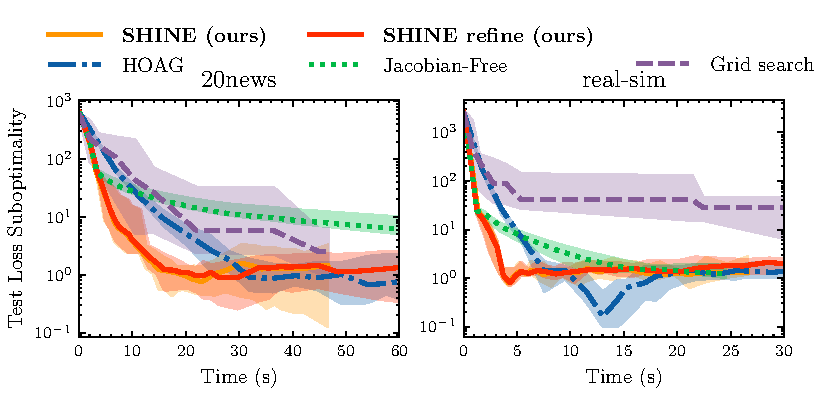
\includegraphics[width=\textwidth]{bilevel_test.pdf}\\

        \strongpoint{Theoretically grounded, can be further refined,\\large scale experiments on DEQs.}
    }



    \section{Algorithm Unrolling}
    \parttitleframe[Differentiable inner problem solvers]{Shaban2019,Ablin2020,Malezieux2022}


    \frame{
        \frametitle{Differentiable unrolling of $\theta^t$}

        {\bf Idea:} \parbox[t]{.9\textwidth}{
            Compute $\frac{\partial \theta^t}{\partial \lambda}(\lambda) \approx \frac{\partial \theta^*}{\partial \lambda}(\lambda)$
            using automatic differentiation\\
            through an iterative algorithm.}\\[2em]

            \visible<2->{
                For the gradient descent algorithm:
                \[
                    \theta^{t+1} = \theta^{t} - \rho \frac{\partial G}{\partial \theta}(\lambda, \theta^t)
                \]
                The Jacobian reads,
                \[
                    \frac{\partial \theta^{t+1}}{\partial \lambda}(\lambda) = \Big(Id - \rho\frac{\partial^2 G}{\partial \theta^2}(\lambda, \theta^t) \Big)\frac{\partial \theta^t}{\partial \lambda}(\lambda) - \rho\frac{\partial^2 G}{\partial \theta\partial \lambda}(\lambda, \theta^t)
                \]
            }
            \visible<3->{
                \strongpoint{Under smoothness conditions, if $\theta^t$ converges to $\theta^*$,\\this converges toward $\frac{\partial \theta^*}{\partial \lambda}(\lambda)$}
            }
    }

    \frame{
        \frametitle{Analysis for min-min problems \rightcite{Ablin et al. 2020}}

        {\bf Context: } min-min problems where $F=G$\\
        \strongpoint{Here, $\frac{\partial F}{\partial \theta}(\lambda, \theta^*)= 0$}
        \vskip1em


        \visible<2->{
        We consider the $3$ gradient estimates:
        \begin{itemize}
            \item  $g_1 = \frac{\partial G}{\partial \lambda} (\lambda, \theta^t)$ \keypoint{Analysis}
            \item  $g_2 = \frac{\partial G}{\partial \lambda} (\lambda, \theta^t)
                + \frac{\partial G}{\partial \theta}(\lambda, \theta^t)\frac{\partial \theta^t}{\partial \lambda}
            $\keypoint{Automatic}
            \item  $g_3 = \frac{\partial G}{\partial \lambda}(\lambda, \theta^t)
            - \frac{\partial G}{\partial \theta}(\lambda, \theta^t)\frac{\partial^2G}{\partial \theta^2}^{-1}(\lambda, \theta^t) \frac{\partial^2 G}{\partial \theta\partial\lambda}(\lambda, \theta^t)
            $\keypoint{Implicit}
        \end{itemize}
        }
        \vskip2em
        \visible<3->{
            \begin{columns}
            \column{.55\textwidth}
            {\bf Convergence rates:} For G strongly convex in $\theta$,
            \begin{align*}
                |g^1_t(x) - g^*(x)| &= O\left(|\theta^t(\lambda)  - \theta^*(\lambda) |\right), \\
                |g^2_t(x) - g^*(x) | &= o\:\left(|\theta^t(\lambda)  - \theta^*(\lambda) |\right), \\
                |g^3_t(x) - g^*(x) | &= O\left(|\theta^t(\lambda)  - \theta^*(\lambda) |^2\right)  .
            \end{align*}
            \column{.4\textwidth}
            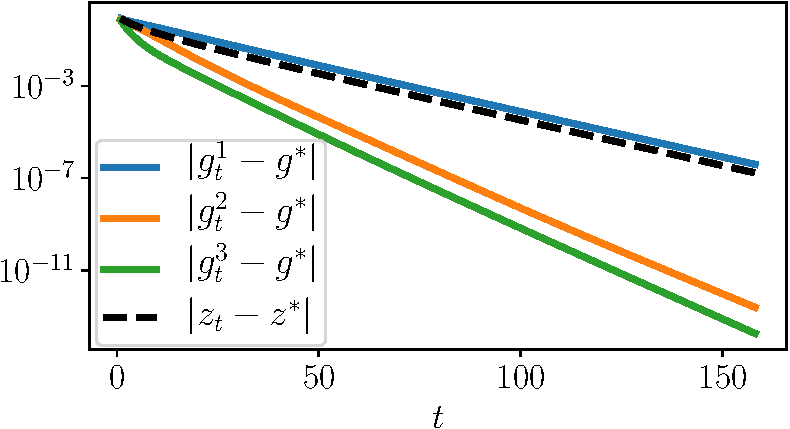
\includegraphics[width=\linewidth]{cvg_gradient}
            \end{columns}
        }

    }

    \frame{
        \frametitle{Analysis for non-smooth min-min problems \rightcite{Malezieux et al. 2022}}

        {\bf Context: } \parbox[t]{.8\textwidth}{dictionary learning, $F=G$ with an $\ell_1$-regularization for $\theta$.}

        \vskip2em
        {\bf Issue: } The implicit gradient quality mostly depends on the support identifiaction,
        \[
            {\Big(\frac{\partial\theta^*}{\partial D_l}\Big)}_{S^*} = -(D_{:, S^*}^\top D_{:, S^*})^{-1}(D_l {\theta^*}^\top + (D_l^\top \theta^* - y_l) Id_n)_{S^*} \enspace ,
        \]
        \vskip2em
        \strongpoint{Is the autodiff approach better than the analytic one?}
    }
    \frame{
        \frametitle{Analysis for non-smooth min-min problems \rightcite{Malezieux et al. 2022}}
        On the support, the function is smooth and we recover the same convergence.\\[1em]
        {\centering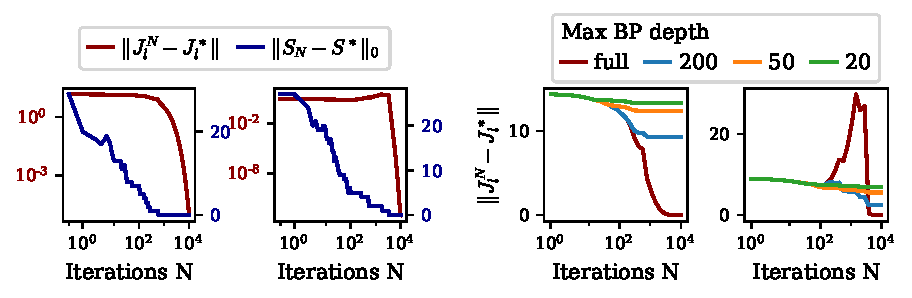
\includegraphics[trim={2.1em 2em 22em 1em}, clip, width=.8\textwidth]{conv_jac}\\}
    }

    \frame{
        \frametitle{Analysis for non-smooth min-min problems \rightcite{Malezieux et al. 2022}}
        Outside of the support, errors can accumulate and the gradient can blow up.\\[1em]
        {\centering 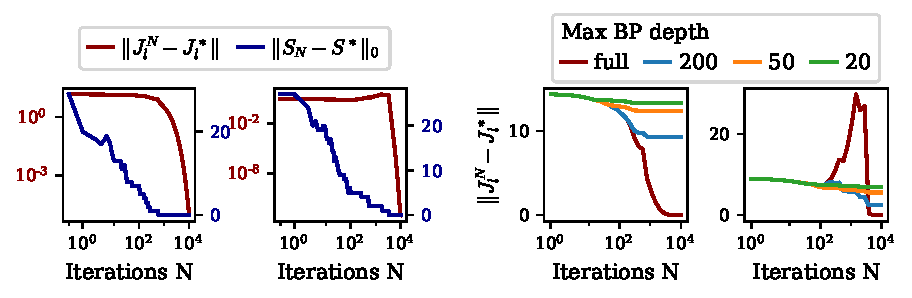
\includegraphics[trim={20.8em 2em .4em .5em}, clip, width=.8\textwidth]{conv_jac}\\
        }

    }

    \frame{
        \frametitle{Conclusion}

        \vspace{0pt plus 1 filll}
        \begin{itemize}
            \item Bi-level optimization is intrinsic in many ML problems.
            \item Classical optimization method can be used once we know how to compute the gradient.
            \item The gradient can be computed either using implicit function theorem or algorithm unrolling.
            \item No clear winner, this depends on the problem at end!
        \end{itemize}


        \vspace{0pt plus 1 filll}
        {\bf Current work:}
        \begin{itemize}
            \item Efficient and stochastic bi-level solvers,
            \item Application of bi-level solvers to Data-Augmentation problems for EEG.
        \end{itemize}
        \vskip-1em
        \strongpoint{Stay tuned!}

        \vspace{0pt plus 1 filll}
        Slides will be on my web page:\\[.5em]
        \hskip5em\includegraphics[height=.8em]{website} \url{tommoral.github.io}
        \hskip4em 
\includegraphics[height=.8em]{twitter} \href{https://twitter.com/tomamoral}{@tomamoral}

        }

        \frame{
            \frametitle{Thanks to all my bi-level collaborators!}
            {\centering
            \includegraphics[height=5em]{People/zramzi}
            \includegraphics[height=5em]{People/sbai}
            \includegraphics[height=5em]{People/fmannel}
            \includegraphics[height=5em]{People/pciuciu}\\[2em]
            \includegraphics[height=5em]{People/pablin}
            \includegraphics[height=5em]{People/gpeyre}\hskip10ex
            \includegraphics[height=5em]{People/bmalezieux}
            \includegraphics[height=5em]{People/mkowalski}\\[3em]

            \includegraphics[height=5em]{People/crommel}
            \includegraphics[height=5em]{People/jpaillard}
            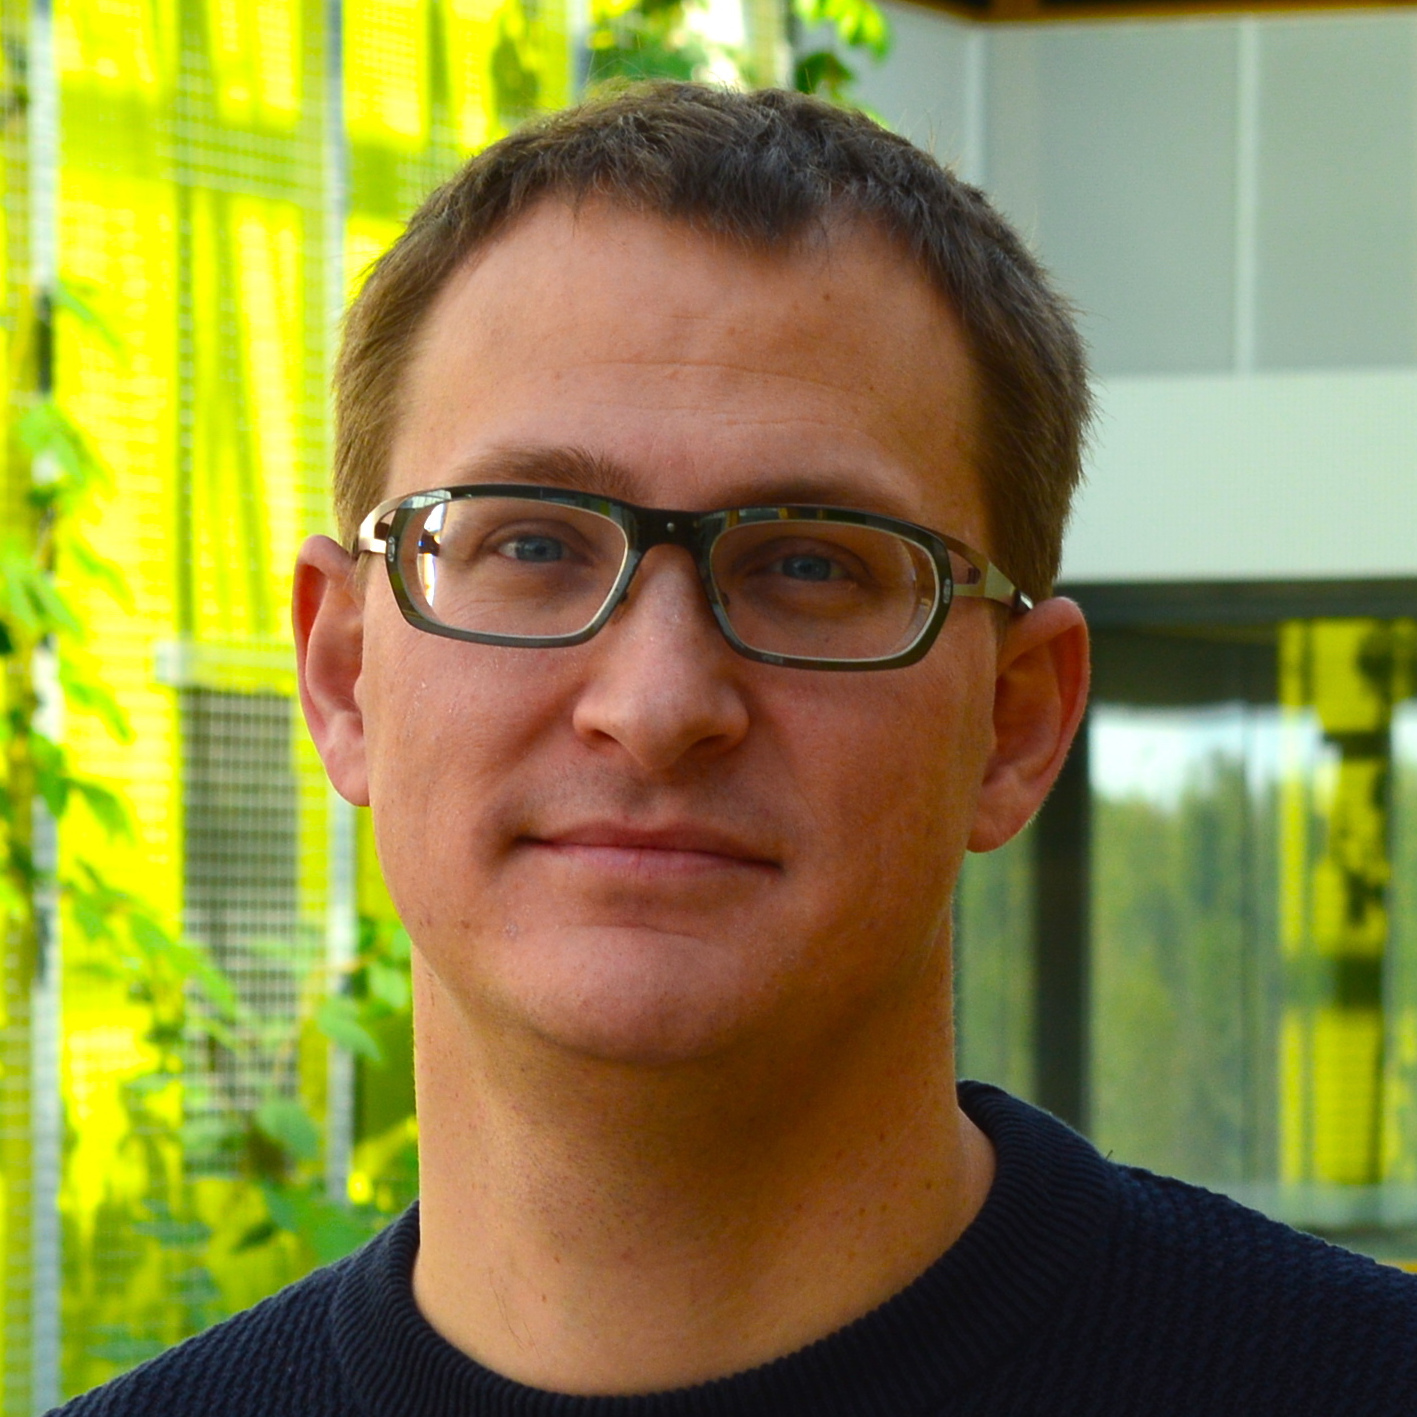
\includegraphics[height=5em]{People/agramfort}
            \includegraphics[height=5em]{People/svaiter}
            \includegraphics[height=5em]{People/mdagreou}\\
            }
        }


\end{document}
